\section{The sample}
\label{sec:sample}

This search covers \NWindows{} spectral windows toward \NStars{}
stars in \NSystems{} systems within 40\,pc, drawn from \NEB{}
public ALMA execution blocks and \TotalDataTB\,TB of raw data through one
frozen pipeline, \StTelHours\,h of telescope time and \LdgCensusHours\,h
summed over windows. That set is the \emph{primary census}, and every limit,
every crossing and every expectation here is computed over it. Three further
sets of blocks enter the paper without being part of it: a hold-out reserved
before any block on its own side of the rule was searched, an archival
extension searched afterwards, and an out-of-sample control beyond 40\,pc. A
fourth, a \emph{rank-calibration sample} drawn from the blocks already counted
above, calibrates the spatial statistic.
Table~\ref{tab:blockledger} names all five in rows that sum, and sets beside
them every count of windows, crossings, systems and bandwidth this paper
quotes, each with the set it counts. Wherever a number here is computed over
something other than the primary census, that table's name for it is used at
the point of use.

\emph{Star} means one stellar component, \emph{system} a bound group
counted once however many of its components were observed, and \emph{target}
one ALMA pointing.

The census is two experiments. \NWinA{} windows toward
\LdgClassAStars{} stars in \NSysClassA{} systems are fine-channel ---
\emph{Class~A} throughout --- and resolve a drifting carrier; every
sensitivity and every exclusion quoted here refers to them unless stated
otherwise. The remaining \NWinB{} are coarse-channel, \emph{Class~B}, and
support a secondary search for unresolved spectral excess, which cannot
distinguish a drifting signal from a stationary one.

The inclusion criteria were applied by query. A star enters
if its Gaia~DR3 parallax is at least 25\,mas, measured to better than
\PlxAdqlPct{} per cent, and if its proper-motion-corrected position at the
observation epoch falls inside the quoted field of view of at least one
public execution block. Distances are direct inversions, $d=1/\varpi$, and
the star need not sit at the pointing centre. One further rule applies to the
window and not to the star: a window is kept only where the primary-beam
response at the star is at least \PbFloorResp. It removes \EpsEriNOffAxis{}
windows, all of them $\epsilon$~Eridani in Band~6, and no others; that band
was then set aside as a whole, and Appendix~\ref{app:conventions} reports its
limits in one place, including the \EpsEriNOnAxis{} windows that place the
star at the pointing centre and pass the floor. None of them enters a census
statistic. The parallax
criterion never binds: the worst fractional parallax error among the stars
searched is \SfPlxWorstPct{} per cent, inside even the stricter
$\sigma_\varpi/\varpi\le\SfPlxCutDec$ of Table~\ref{tab:selfunc}'s
reference census. The query returns
\NCensus{} work-list entries; the quoted field of view is optimistic, and
only \NGenuinelyCovered{} of those stars are in fact contained by a public
field, of which \NStars{} yielded a searchable window. One target has no
catalogue name --- a serendipitous field star that appears throughout as
\BkAlmaName, Gaia~DR3 \BkAlmaGaia, an \BkAlmaSpType{} dwarf at
\BkAlmaDistPc\,pc with no measured systemic velocity.

Disc, planet and colour enter as descriptive metadata only, and no
star was excluded by any criterion other than the three above. Three removals
act on windows instead, and account for the whole difference between the
\LqNExport{} rows the extraction wrote and the \NWindows{} retained:
\NDup{} repeated rows of one window, the \NWithheld{} withheld above, and
\NDefect{} windows failing a quality cut that is physical rather than chosen.
Since $\sigma\sqrt{t_{\rm on}\Delta\nu_{\rm ch}}$ is set by system
temperature and collecting area, a window more than \LqDefectCut{} times
below the sample median in it is not measuring the sky; those removed lie
$\LqDefectFacLo$--$\LqDefectFacHi$ times below it and the nearest retained
\LqKeptFac{} times, so the threshold's value does not matter. No
integration-time cut was applied; the shortest window retained carries
\LqOnsrcMin\,s on source.

\subsection{The archival selection}
\label{sec:bias}

This sample was not designed: it is whatever previous ALMA programmes
happened to observe, and \PctDiscProposal{} per cent of the stars searched
were targeted under a debris-disc or planet-formation proposal.
Table~\ref{tab:selfunc} measures the bias against a volume-limited reference
census of which the searched stars are a subset, classifying both columns by
one rule --- BP$-$RP colour with the absolute G magnitude, which reaches
\SfCensusColPct{} per cent of the census and \SfClassifiedPct{} per cent of
the searched sample --- so every ratio below is like against like.

The dominant selection effect is distance. Stars within 5\,pc are
over-represented by a factor \SfTopRatio, and the enhancement falls
monotonically with distance to a factor of two \emph{under}-representation
beyond 30\,pc. Colour comes second: A~stars are over-represented by about
\SfARatio{} and F and G stars by factors of three, because those are the
stars with bright debris discs. M~dwarfs are depleted ---
\SfMSearched{} of the \SfNStar{} searched stars are M~dwarfs, a factor
\SfMRatio{} of their share of the reference census, and only
\SfMClassAStars{} of them carry the fine-channel coverage that can resolve a
drifting carrier at all. Coverage is also concentrated:
\ConcThreeWin{} of the \NWindows{} windows come from \ConcThreeSys{}
systems. Every statistical statement in this paper is therefore a statement
about an archive-selected sample of nearby stars, and none of them is an
occurrence rate for the solar neighbourhood. The selection acts hardest on
exactly the targets a designed search would pick: of the \CsIntNRow{} sample
systems within 15\,pc with a confirmed planet, \CsIntNoClassA{} carry no
Class~A coverage and so no drift-resolving limit.

%% GENERATED by selfunc_v411.py -- do not hand-edit.
\begin{table}
\centering
\scriptsize
\setlength{\tabcolsep}{4pt}
\caption{Selection function of the searched sample against a volume-limited reference census. Both columns are the same Gaia~DR3 selection --- $\varpi>0$, $\sigma_\varpi/\varpi\le0.1$ and $1/\varpi\le40$\,pc, 17\,566 objects --- of which the 89 searched stars are rows, so the two are selected alike by construction; and both are classified by one rule, in which BP$-$RP colour sets the class and the absolute G magnitude separates the degenerates that colour alone would place among the A~stars. The rule reaches 17\,278 census objects and 87 of the 89 searched stars, the rest carrying no Gaia BP or RP photometry. ``Ratio'' is the searched column fraction over the census column fraction; $>1$ is over-representation. The strongest selection effect here is distance, not colour.}
\label{tab:selfunc}
\begin{tabular}{@{}lrrr@{}}
\toprule
Property & Census & Searched & Ratio \\
\midrule
\multicolumn{4}{@{}l}{Distance} \\
\quad $d\le5$\,pc & 48 (0.3\%) & 12 (13.5\%) & 49.3 \\
\quad 5--10\,pc & 240 (1.4\%) & 13 (14.6\%) & 10.7 \\
\quad 10--20\,pc & 2069 (11.8\%) & 18 (20.2\%) & 1.7 \\
\quad 20--30\,pc & 5391 (30.7\%) & 19 (21.3\%) & 0.7 \\
\quad 30--40\,pc & 9818 (55.9\%) & 27 (30.3\%) & 0.5 \\
\midrule
\multicolumn{4}{@{}l}{Colour class$^{a}$} \\
\quad A & 61 (0.4\%) & 5 (6.3\%) & 17.4 \\
\quad F & 473 (2.8\%) & 8 (10.1\%) & 3.6 \\
\quad G & 978 (5.8\%) & 15 (19.0\%) & 3.3 \\
\quad K & 2221 (13.2\%) & 10 (12.7\%) & 1.0 \\
\quad M & 13\,082 (77.8\%) & 41 (51.9\%) & 0.7 \\
\midrule
\multicolumn{4}{@{}l}{Other axes} \\
\quad Confirmed planet hosts$^{b}$ & 26 (15.5\%) & 23 (25.8\%) & 1.7 \\
\quad White dwarfs$^{a}$ & 463 (2.7\%) & 8 (9.0\%) & 3.4 \\
\quad Searched stars / systems & -- & 89 / 82 & -- \\
\bottomrule
\end{tabular}

\smallskip
{\footnotesize $^{a}$Colour bins, not MK types. The boundaries are the colours at which the census's own temperature--colour relation crosses 7500, 6000, 5300 and 3900\,K: BP$-$RP $<0.36$ for A, 0.36--0.72 for F, 0.72--0.95 for G, 0.95--1.77 for K and $>1.77$ for M. Over the 8594 census objects that also carry a Gaia temperature the two classifications agree for 98 per cent, and every disagreement is between neighbouring bins. A star is counted as degenerate when it lies more than 4\,mag below the main sequence measured from the census itself: the two sequences are separated by 5 to 8\,mag here, so moving the cut by a magnitude either way changes the count by under 3 per cent. The five classes are normalised over the 79 non-degenerate searched stars and the 16\,815 non-degenerate census objects.\\ $^{b}$Both columns are the same positional join, of the 168-entry ALMA-covered work list and of its searched subset, to the NASA Exoplanet Archive \texttt{pscomppars} table accessed 2026 October 4. The 23 searched hosts carry 50 confirmed planets, 21 of the 23 surviving the deuterium-burning mass limit; the Gaia census carries no planet information, so the census column in this row is the work list and not the 17\,566-object Gaia census.}
\end{table}


%% fig:funnel DELETED: it drew the three counts the sentence above it
%% already carries, so it joined the prose instead of replacing it.  The
%% artwork is online material (figures_diagnostic/selection_funnel.pdf).

\subsection{Frequency coverage and archival scope}
\label{sec:coverage}

The Class~A experiment covers $\Delta\nu_A=\DnuA$\,GHz of unique sky
frequency, and that coverage is sparse: \DomAIslands{} disjoint islands
scattered between \DomAFreqLo{} and \DomAFreqHi\,GHz, not a band, so the
endpoints are a range over which observations exist and never one that was
covered. Adding the coarse-channel windows brings the total archival coverage
to \DnuAB\,GHz in \UnionIntervals{} intervals, of which \SearchedUnionGHz\,GHz
survives the molecular-line mask of \S\ref{sec:method}.
Fig.~\ref{fig:waterfall} shows the distribution; a transmitter at a frequency
between the islands was never observable here, whatever its power.

The archive is not exhausted either, and the shortfall is accounted for.
\LdgExtScope{} further blocks lie inside the same query but were not
processed when the census was frozen. \LdgExtSearched{} have since been
calibrated and searched, \LdgExtEB{} of them reported here as repeat epochs
and as a sample the frozen pipeline had not seen; the other
\BkExtNotReported{} enter no number anywhere, for the reasons
Table~\ref{tab:blockledger} gives row by row. The largest single gap is the
\FateNoCal{} blocks whose raw visibilities the archive holds but never
pipeline-calibrated, \FateNoCalGB\,GB in all; no effort of ours would close
it.

\begin{figure*}
\centering
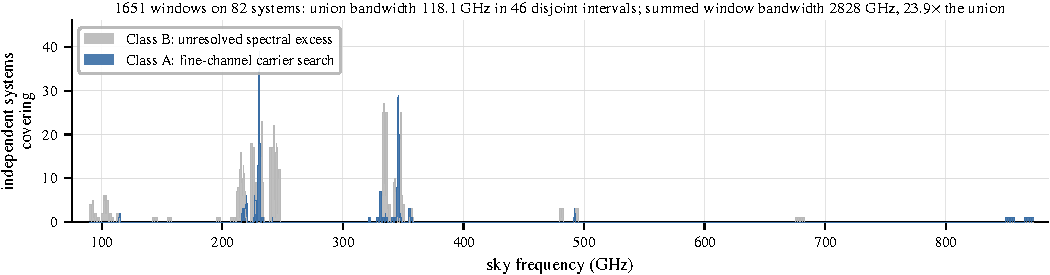
\includegraphics[width=0.99\textwidth]{figures/coverage_waterfall.pdf}
\caption{Where this survey searched. \emph{Lower panel:} each searched
window is a horizontal segment on its host system's row, rows ordered by
distance; heavy blue marks the fine-channel carrier search (Class~A) and
light grey the coarse-channel spectral-excess search (Class~B).
\emph{Upper panel:} the number of systems covering each gigahertz of sky
frequency. The summed window bandwidth is $\GrossOverUnion\times$ the union,
so the union measures frequency coverage and the summed bandwidth search
effort.}
\label{fig:waterfall}
\end{figure*}

%% Floats that belong elsewhere: tab:blockledger is in Appendix A (its
%% headline rows are in the prose above, so the cross-reference is not a
%% pointer with no numbers beside it); tab:interesting is neither typeset nor
%% distributed -- r15-deposit, 2026-10-08: there is no deposit, so if its rows
%% are wanted by a reader they have to be printed; tab:searchspace is deleted, nothing having cited
%% it, and its counts, unions, channel widths and drift range are all
%% elsewhere in the paper.
%% Carried forward to the numbers owner: tab_interesting.tex is still
%% generated but is not in make_all.sh, and its planet column should read the
%% dated NASA Exoplanet Archive extract selfunc_v411.py uses so that one
%% definition of "confirmed planet" serves both tables.  Two display defects
%% belong in star_alias.designation: Barnard's Star prints as a SIMBAD
%% identifier with the "NAME" prefix stripped, and BD+05 1668 would read
%% better with its GJ alias beside it.
